% Copyright (C) 2006 Thomas L. Kula
% All Rights Reserved
%
% See the file LICENSE for license terms.
\documentclass[12pt]{article}
\usepackage{graphicx}
\setlength{\paperwidth}{5.5in}
\setlength{\paperheight}{8.5in}
\setlength{\textheight}{6.45in}
\setlength{\oddsidemargin}{-0.5in}
\setlength{\evensidemargin}{-0.5in}
\setlength{\textwidth}{4.0in}
\setlength{\parindent}{0in}
\setlength{\parskip}{3mm}
\usepackage[print]{booklet} \nofiles
\source{\magstep0}{5.5in}{8.5in}
\target{\magstep0}{11in}{8.5in}
\setpdftargetpages
\begin{document}

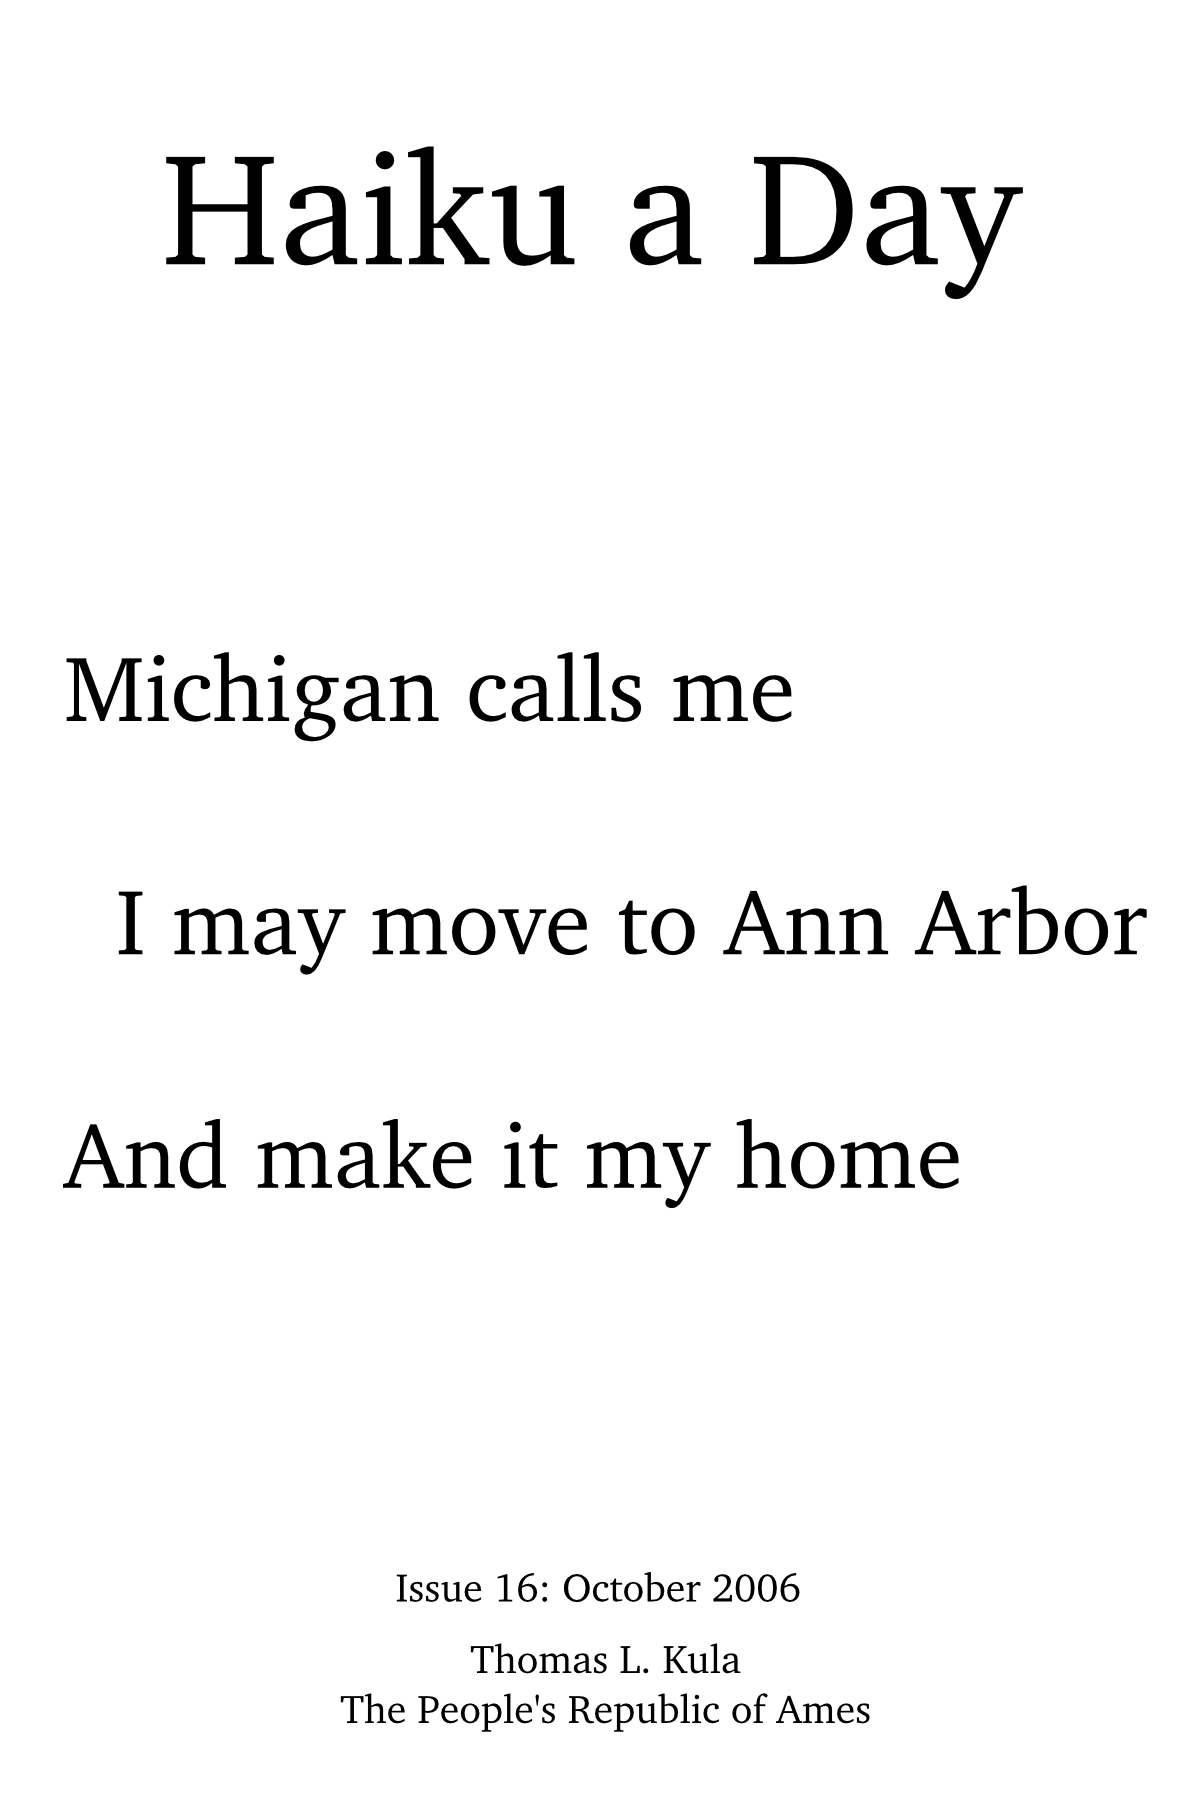
\includegraphics[width=101mm]{frontpage.png}

\newpage

Well, folks, after nearly six years in Ames it looks
like I will be moving. For a while I've been looking
around for another job, something that was more in 
line with what I wanted to do. And now, I've been
offered a position at the University of Michigan.
So, baring any miracle on the part of ISU, I will be
moving by the end of the month --- and let me tell
you, moving does not fill me with much joy. But I'm
sure I'll survive. I think it's the only way I'll
ever get my garage cleaned out.

So, by this time next month, your Haiku a Day may 
appear from The People's Republic of Ames, newly
located in Ann Arbor. We'll see what happens.

--- Thomas

http://kula.tproa.net/had/ \\
kula@tproa.net

Downloadable version available at website, or if you really
want me to send you one, send me your address, maybe a
stamp too. I enjoy getting mail as much as I enjoy sending
mail. Of course, I have no idea what my address may be at
this point....

\setlength{\parskip}{1mm}

1 October 2006

Clatter of the train \\
Shuffling by as I awake \\
Mile long alarm


\newpage

2 October 2006

October Eighties \\
The weather here is screwed up \\
It should be cold now

3 October 2006

Goodbye poor laptop \\
Your mobo is sad again \\
Welcome new macbook

4 October 2006

Sleep is for the weak \\
You foolishly say and then \\
Get insomnia

5 October 2006

Oh that Thursday joy \\
The weekend will be here soon \\
Some friends will visit

6 October 2006

Casa del JaBeth \\
Made ready for Star Trek Night \\
I have pizza rolls

7 October 2006

The Eighth Star Trek Night \\
Eighteen hours of madness \\
Show me Kirk Unit



\newpage

8 October 2006

Star Trek Night over \\
This year was easy for me \\
My mettle is strong

9 October 2006

My office carpet \\
Thin, green and somewhat threadbare \\
It needs vacuuming

10 October 2006

Kaki King smiles \\
Beautiful tunes float on by \\
And I become peace

11 October 2006

Little flakes of snow \\
Dancing gaily in the wind \\
Skitter down to Earth

12 October 2006

To my parent's house \\
An evening at the old home \\
The couch is not soft

13 October 2006

Visit Madison \\
An interview there goes well \\
You should hire me


\newpage

14 October 2006

I have found Nesbitts \\
Honey lemonade delights \\
The gods' own nectar

15 October 2006

Wind blows against me \\
My legs unridden too long \\
Slow going by bike

16 October 2006

Madison likes me \\
Another chance to visit \\
And get more cheese curds

17 October 2006

Waking while it's dark \\
Fine when you go back to sleep \\
Not going to work

18 October 2006

Habeus Corpus \\
O Sic Transit Gloria \\
You had a good run

19 October 2006

The rice has fallen \\
The container was not sealed \\
Tasty food scatters


\newpage


20 October 2006

The clothes rod falls down \\
Laundry bops me on the head \\
Clean shirt avalanche

21 October 2006

Books, glorious books \\
A shelf haphazardly full \\
A clutter of joy!

22 October 2006

Madison again \\
I can see the Capitol \\
From my hotel room

23 October 2006

Another long drive \\
Some tunes keep me company \\
Heater keeps me warm

24 October 2006

College algebra \\
A book of mathematics  \\
Numbers dance for me

25 October 2006

Yay! Cheap pizza day! \\
Half a pineapple, all mine \\
Burp down with soda


\newpage

      
26 October 2006

The sleepy is strong \\
Office naps do not work well \\
I need a couch here

27 October 2006

A crisp fall evening \\
Leaves skitter as the wind blows \\
The sigh of autumn. 

28 October 2006
 
Into the aether \\
"Monster Mash" is sure to make \\
Confused aliens 

29 October 2006

Skater wizzes by \\
Wheels clack on cracks in the road \\
Scraping on asphalt

30 October 2006

Willies from the past \\
The War of the Worlds broadcast \\
Orson Welles is good

31 October 2006

Large bowl of candy \\
Just a few trick-or-treaters \\
Guess I'm eating it

\newpage


\includegraphics[width=101mm]{backpage.png}

\end{document}




